% Created 2020-10-26 Mon 12:43
% Intended LaTeX compiler: pdflatex
\documentclass[presentation, aspectratio=169]{beamer}
\usepackage[utf8]{inputenc}
\usepackage[T1]{fontenc}
\usepackage{graphicx}
\usepackage{grffile}
\usepackage{longtable}
\usepackage{wrapfig}
\usepackage{rotating}
\usepackage[normalem]{ulem}
\usepackage{amsmath}
\usepackage{textcomp}
\usepackage{amssymb}
\usepackage{capt-of}
\usepackage{hyperref}
\RequirePackage{fancyvrb}
\usepackage[margin=0.5in]{geometry}
\usepackage[backend=bibtex]{biblatex}
\addbibresource{./../biblio.bib}
\author[A. Caliò]{Antonio Caliò\inst{1}}
\usetheme{default}
\date{}
\title{Introduction to Scala}
\institute{\inst{1}DIMES Dept., University of Calabria\\ Rende (CS), IT \\ a.calio@unical.it\\ Big Data Analytics - Computer Engineering for the IoT}
\titlegraphic{\begin{picture}(0,0) \put(200,200){\makebox(0,0)[rt]{
\includegraphics[width=3cm]{./img/logo_dimes.jpg}}} \end{picture}}}
\AtBeginSection[]{\begin{frame}<beamer>\frametitle{Presentation agenda}\tableofcontents[currentsection]\end{frame}}
\hypersetup{
 pdfauthor={},
 pdftitle={Introduction to Scala},
 pdfkeywords={},
 pdfsubject={},
 pdfcreator={Emacs 27.1 (Org mode 9.3)}, 
 pdflang={English}}
\begin{document}

\maketitle
\begin{frame}{Outline}
\tableofcontents
\end{frame}





\section{Introduction}
\label{sec:orgb552187}

\begin{frame}[label={sec:orgbb2abf2}]{What is Scala}
\begin{itemize}
\item \alert{Scala} stands for: \emph{scalable language}.
\item It combines object-oriented programming with
functional programming
\item A Scala program runs on a JVM.
\item Scala can execute Java Code -- thus, Scala understands Java code
\item As an object-oriented language, we can define classes and class hierarchies via the inheritance
\item As a functional language Scala provides lightweight syntax for defining \emph{anonymous functions} -- like Java lambdas -- 
it also allows the definition of nested functions
\item Scala is \emph{statically} typed  like many other programming languages (e.g. C, Pascal, Rust). 
Nonetheless, it does not need the programmer to specify the type of a variable
the type information of a variable (most of the times)
\end{itemize}
\end{frame}

\begin{frame}[label={sec:orgf3f1504}]{Setting up your environment}
\begin{enumerate}
\item You must have a working Java environment -- I am sure you already have one on your machine!
\item Install Scala\footnote{It is recommended to install the 2.12 version}. You can either:
\begin{itemize}
\item Download the installer from \href{https://www.scala-lang.org/download/2.12.12.html}{Scala-Lang}
\item If you are on Linux chances are that it is available within you repository
\end{itemize}
\item Download and install the Scala main build-system: \href{https://www.scala-sbt.org/download.html}{SBT}
\end{enumerate}
\end{frame}

\begin{frame}[label={sec:org57426ff},fragile]{You First Scala Program}
 It the installation is successful you should be able to run Scala in 
console mode.
\begin{figure}[htbp]
\centering
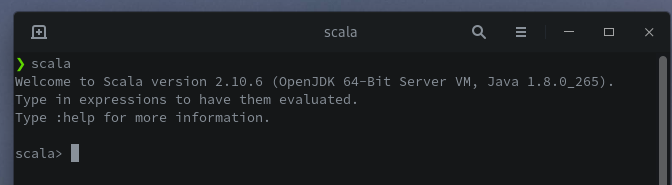
\includegraphics[width=.9\linewidth]{./img/scala-console.png}
\caption{\label{fig:orgccc9a23}Scala Console}
\end{figure}

Then print the usual \texttt{Hello World} string.
\begin{verbatim}
println("Hello World")
\end{verbatim}
\end{frame}


\begin{frame}[label={sec:org84e8ca4},fragile]{Scala in Script Mode}
 \begin{itemize}
\item Create a file: \texttt{HelloWorld.scala}
\end{itemize}
\begin{verbatim}
object HelloWorld {
  def main(args: Array[String]) = {
     println("Hello World")
  }
}
\end{verbatim}
\begin{itemize}
\item Compile with  \texttt{scalac HelloWorld.scala}
\item Run with \texttt{scala HelloWorld}
\end{itemize}
\end{frame}

\section{Basic Syntax}
\label{sec:orga51a80c}

\begin{frame}[label={sec:org88ee854}]{Basic Concepts}
\begin{itemize}
\item Scala is Case Sensitive
\item Class names should be in upper case
\item Method names should start with lower letters
\item Program file names should match the name of the object
\item Every Scala program must have a main function
\end{itemize}
\end{frame}

\begin{frame}[label={sec:orga4813bd},fragile]{Scala Identifiers}
 Every Scala component requires a name. 

Names are used for objects, classes, variables and methods.
There are four types of identifier:
\begin{itemize}
\item Alphanumeric identifier, e.g., \texttt{age}, \texttt{salary}, \texttt{\_age1}, \texttt{\_\_1\_value}
\item Operator identifier, e.g., \texttt{+, ++, :::, =>}. The scala compiler will mangle this operators 
by turning them into a correspondent Java identifier
\item Mixed identifier. It is an alphanumeric identifier followed by an underscore and an operator identifier.
For instance: \texttt{var\_+, var\_=}.
\item Literal identifier. It is an arbitrary string enclosed within a pair of ``.
\end{itemize}
\end{frame}

\begin{frame}[label={sec:org95a70b3},fragile]{Scala Packages}
 \begin{itemize}
\item In order to declare a package, in the first non-comment line in the file you should write:
\begin{verbatim}
package name.of.the.package
\end{verbatim}

\item We can import the entire scope of a package as follows:
\begin{verbatim}
import scala.xml._
\end{verbatim}
the underscore is equivalent to * in Java

\item A single class is imported as follows:
\begin{verbatim}
import scala.collection.mutable.HashMap
\end{verbatim}

\item You can also import multiple class as follow:
\end{itemize}
\begin{verbatim}
import scala.collection.immutable.{TreeMap, TreeSet}
\end{verbatim}
\end{frame}


\begin{frame}[label={sec:org8c7c594},fragile]{Scala Type Dynamic}
 \begin{itemize}
\item A \texttt{Dynamic} is a marker trait/interface that enables dynamic invocations. 
Therefore is a variable \texttt{x} is an instance of an object adhering to the \texttt{Dynamic} interface.

\item There are four different types of dynamics:
\begin{enumerate}
\item \texttt{selectDynamic} it allows to write field accessors: \texttt{x.foo}

\item \texttt{updateDynamic} it allows to write field update: \texttt{x.foo = 5}

\item \texttt{applyDynamic} it allows to call methods with arguments: \texttt{x.bar(0)}

\item \texttt{applyDynamicNamed} it allows to call methods with named arguments: \texttt{x.bar(y=8)}
\end{enumerate}

\item In order to define a class adhering to this specifications you just need to extends 
the \texttt{Dynamic} interface:
\end{itemize}

\begin{verbatim}
import scala.language.dynamics
class MyClass extends Dynamic{ 
}
\end{verbatim}
\end{frame}


\begin{frame}[label={sec:org5ed76b8},fragile]{Select Dynamic}
 \begin{verbatim}
class DynImpl extends Dynamic {
  def selectDynamic(name: String) = name
}
\end{verbatim}
Try:
\begin{verbatim}
val d = new DynImpl()
d.foo 
d.selectDynamic("foo")
\end{verbatim}
\end{frame}


\begin{frame}[label={sec:org0918bd1},fragile]{Update Dynamic}
 \begin{verbatim}

class DynImpl extends Dynamic {

  var map = Map.empty[String, Any]

  def selectDynamic(name: String) =
    map get name getOrElse sys.error("method not found")

  def updateDynamic(name: String)(value: Any) {
    map += name -> value
  }
}
\end{verbatim}
Try:
\begin{verbatim}
val d = new DynImpl
d.foo 
d.foo = 10
d.foo
\end{verbatim}
\end{frame}

\begin{frame}[label={sec:orgd6ddb2f},fragile]{Apply Dynamic}
 \begin{verbatim}
class DynImpl extends Dynamic {
  def applyDynamic(name: String)(args: Any*) =
    s"method '$name' called with arguments ${args.mkString("'", "', '", "'")}"
}
\end{verbatim}
Try:
\begin{verbatim}
val d = new DynIml
d.ints(1,2,3)
\end{verbatim}
\end{frame}

\begin{frame}[label={sec:org3f1e070},fragile]{Apply Named Dynamic}
 \begin{verbatim}
class DynImpl extends Dynamic {
  def applyDynamicNamed(name: String)(args: (Strin,Any)*) =
    s"method '$name' called with arguments ${args.mkString("'", "', '", "'")}"
}
\end{verbatim}
Try:
\begin{verbatim}
val d = new DynIml
d.ints(i1=1,i2=2,i3=3)
\end{verbatim}
\end{frame}



\section{Variables}
\label{sec:orgc857d69}

\begin{frame}[label={sec:orgefca510},fragile]{val vs var}
 A variable can be defined as: 
\begin{itemize}
\item a value, with the \texttt{val} keyword. These are constants
\item a variable,  with the \texttt{var} keyword. These are mutable
\end{itemize}
\end{frame}


\begin{frame}[label={sec:orgc16784c},fragile]{Declaring a variable}
 \begin{itemize}
\item The syntax to declare a new variable is the following:
\begin{verbatim}
val myVar: String = "Foo"
\end{verbatim}

\begin{itemize}
\item It is the syntax rule:
\end{itemize}
\end{itemize}
\begin{verbatim}
[val|var] <variableName> {: <dataType>} = <Initial Value>
\end{verbatim}

\begin{itemize}
\item Scala has also a mechanism for type inference, so you do not need to specify the 
type of the variable
\end{itemize}
\begin{verbatim}
val myVal = "Hello"
var myVar = 4
\end{verbatim}
\end{frame}
\begin{frame}[label={sec:orgada4a43},fragile]{Example Program}
 \begin{verbatim}
object Demo {
   def main(args: Array[String]) {
      var myVar :Int = 10
      val myVal :String = "Hello Scala with datatype declaration."
      var myVar1 = 20
      val myVal1 = "Hello Scala new without datatype declaration."

      println(myVar)
      println(myVal)
      println(myVar1)
      println(myVal1)
   }
}
\end{verbatim}
\end{frame}

\begin{frame}[label={sec:orga5da840}]{Variable Scope}
Three possible scopes:
\begin{itemize}
\item Field - a field is a variable defined within the scope of an object.
It is accessible both from inside the object and from inside the object.
\item Method Parameter - it is always an immutable object, it is accessible only from 
inside the method it is passed to
\item Local Variable - it accessible only from inside the method. Except for 
returned object
\end{itemize}
\end{frame}

\section{Custom Data Types}
\label{sec:org3856197}

\begin{frame}[label={sec:org44f897e},fragile]{Basic Class}
 \tiny
\begin{verbatim}
class Point(xc: Int, yc: Int) {
   var x: Int = xc
   var y: Int = yc

   def move(dx: Int, dy: Int) {
      x = x + dx
      y = y + dy
      println ("Point x location : " + x);
      println ("Point y location : " + y);
   }
}

object Demo {
def main(args: Array[String]) = {
   val pt = new Point(10,20)
   pt.move(10, 10)
  }
}
\end{verbatim}
\end{frame}

\begin{frame}[label={sec:orgd24c411},fragile]{Extending a class}
 \tiny

\begin{columns}
\begin{column}{0.45\columnwidth}
\begin{verbatim}
import java.io._

class Point(val xc: Int, val yc: Int) {
   var x: Int = xc
   var y: Int = yc

   def move(dx: Int, dy: Int) {
      x = x + dx
      y = y + dy
      println ("Point x location : " + x);
      println ("Point y location : " + y);
   }
}

class Location(override val xc: Int, override val yc: Int,
   val zc :Int) extends Point(xc, yc){
   var z: Int = zc

   def move(dx: Int, dy: Int, dz: Int) {
      x = x + dx
      y = y + dy
      z = z + dz
      println ("Point x location : " + x);
      println ("Point y location : " + y);
      println ("Point z location : " + z);
   }
}

\end{verbatim}
\end{column}
\begin{column}{0.45\columnwidth}
\begin{verbatim}

object Demo {
   def main(args: Array[String]) {
      val loc = new Location(10, 20, 15);

      // Move to a new location
      loc.move(10, 10, 5);
   }
}
\end{verbatim}
\end{column}
\end{columns}
\end{frame}
\begin{frame}[label={sec:org1fde4b7},fragile]{Implicit Classes}
 Implicit classes are very useful as they allow implicit conversions with class's primary constructor
when the class is in scope.

They can be declared as follows:
\begin{verbatim}
object <object name>{
  implicit class <class name> (<Variable>: Data type) {
    def <method>(): Unit = {}
  }
}
\end{verbatim}
\end{frame}
\begin{frame}[label={sec:org47c4d73},fragile]{Implicit Class Example}
 Here is an example of an implicit class named \texttt{IntTimes}. 

It has method that repeatedly print "Hello" to the screen
\tiny
\begin{verbatim}
object Run {
   implicit class IntTimes(x: Int) {
      //f:=> means that f will be evaluated when it is accessed
      def times [A](f: =>A): Unit = {
	 def loop(current: Int): Unit =
	 if(current > 0){
	    f
	    loop(current - 1)
	 }
	 loop(x)
      }
   }

  def main(args: Array[String]) = {
    //4 is interpreted as a IntTimes object upon which we call the times methods passing the 
    //function prinln
    4 times println("hello")
  }
}
\end{verbatim}
\end{frame}
\begin{frame}[label={sec:org6333ddf},fragile]{Singleton Objects}
 \begin{itemize}
\item Scala is more object-oriented if compared to Java.
\item In Scala a class cannot have static members
\item We can define \texttt{object} as opposed to \texttt{class}. Objects works similarly to java static objects
\item An \texttt{object} is a singleton
\item An \texttt{object} has only the default constructor which is implicitly  called when it gets created
\item Usually objects are used to put the main method of the application
\end{itemize}
\end{frame}


\begin{frame}[label={sec:orgc77d9a4},fragile]{Singleton Object Example - Demo.scala}
 \tiny
\begin{verbatim}
class Point(val xc: Int, val yc: Int) {
   var x: Int = xc
   var y: Int = yc

   def move(dx: Int, dy: Int) {
      x = x + dx
      y = y + dy
   }
}

object Demo {
   def main(args: Array[String]) {
      val point = new Point(10, 20)
      printPoint

      def printPoint{
	 println ("Point x location : " + point.x);
	 println ("Point y location : " + point.y);
      }
   }
}
\end{verbatim}
\end{frame}

\section{Access Modifiers}
\label{sec:org358498d}

\begin{frame}[label={sec:orgf9742bc},fragile]{Private Members}
 It is visible only inside the class or object that contains the member definition.

\begin{verbatim}
class Outer {
  class Inner {
    private def f() { println("f") }
    class InnerMost {
      f() //ok
    }
  }
  (new Inner).f() // Error
}
\end{verbatim}
\begin{itemize}
\item In the above example the first call to f() is legal because the class \texttt{InnerMost} is
declared within the scope of \texttt{Inner}, thus it can see the method.
Outside the \texttt{Inner} scope however, the function remains inaccessible.
\end{itemize}
\end{frame}

\begin{frame}[label={sec:org6486ce7},fragile]{Protected Members}
 A protected member is accessible from every subclass 


\begin{verbatim}
package p {
   class Super {
      protected def f() { println("f") }
   }

   class Sub extends Super {
      f()
   }

   class Other {
      (new Super).f() // Error: f is not accessible
   }
}
\end{verbatim}
\end{frame}

\begin{frame}[label={sec:org60c8c09},fragile]{Public Members}
 A member is public by default -- unless we specify any of the previous keywords.

Public members can be accessed from anywhere in the code

\begin{verbatim}
class Outer {
   class Inner {
      def f() { println("f") }
       class InnerMost { f() } // OK 
   }
   (new Inner).f() // OK because now f() is public
}
\end{verbatim}
\end{frame}

\begin{frame}[label={sec:orga168197},fragile]{Scope of Protection}
 Access modifiers can be augmented. 
For instance we can declare a member with the syntax: \texttt{private[X]}.
This means that the member is private "up to" X, where X can be a package, class or singleton object

\begin{verbatim}
package society {
   package professional {
      class Executive {
	 private[professional] var workDetails = null
	 private[society] var friends = null
	 private[this] var secrets = null

	 def help(another : Executive) {
	    println(another.workDetails)
	    println(another.secrets) //ERROR
	 }
      }
   }
}
\end{verbatim}
\begin{itemize}
\item \texttt{workDetails} is reachable by any class defined within the package \texttt{professional}
\item \texttt{friends} is reachable by any class within the package \texttt{society}
\item \texttt{secrets} is reachable only by the implicit object instance methods
\end{itemize}
\end{frame}

\section{Operators}
\label{sec:org9dcab3a}

\begin{frame}[label={sec:org4f6d93d}]{Operators}
Nothing new here!
\end{frame}

\section{If-Else}
\label{sec:org968bd0f}

\begin{frame}[label={sec:org6539837}]{If-Else}
Nothing new here!
\end{frame}

\section{Loops}
\label{sec:org88ca0f1}

\begin{frame}[label={sec:orgf8e2154},fragile]{Loops}
 There are three different kinds of loop statement:
\begin{enumerate}
\item \texttt{while loop}
\item \texttt{do-while loop}
\item \texttt{for-loop}
\end{enumerate}
\end{frame}

\begin{frame}[label={sec:orged486ee},fragile]{while loop - Nothing Weird}
 \begin{verbatim}
object Demo {
   def main(args: Array[String]) {
      // Local variable declaration:
      var a = 10;

      // while loop execution
      while( a < 20 ){
	 println( "Value of a: " + a );
	 a = a + 1;
      }
   }
}
\end{verbatim}
\end{frame}

\begin{frame}[label={sec:org55a21e7},fragile]{do-while loop - Nothing Weird}
 \begin{verbatim}
object Demo {
   def main(args: Array[String]) {
      // Local variable declaration:
      var a = 10;

      // do loop execution
      do {
	 println( "Value of a: " + a );
	 a = a + 1;
      }
      while( a < 20 )
   }
}
\end{verbatim}
\end{frame}

\begin{frame}[label={sec:org02d19e0},fragile]{for-loop}
 \begin{itemize}
\item For-loop leverages on the notion of range -- very similar to Python.

\item A range is \ldots{} a range! it has a start and an end.
\end{itemize}
\begin{verbatim}
for (i <-1 to 10){
   doSomething()
}
\end{verbatim}
\begin{itemize}
\item the "<-" operator is called \emph{generator}. It generates all the value between both ends in the range
and it assigns them to the variable on the left side.
\end{itemize}
\end{frame}

\begin{frame}[label={sec:org2e637cd},fragile]{multiple ranges}
 You can also use multiple range within the same for-loop as follows:
\begin{verbatim}
for( a <- 1 to 3; b <- 1 to 3)
   println( "a,b: " + a + " " + b  );

\end{verbatim}
It is the same as having two nested loop. 
Thus it is equivalent to having the following loop:
\begin{verbatim}
for( a <- 1 to 3)
  for(b <- 1 to 3)
   println( "a,b: " + a + " " + b  );
\end{verbatim}
\end{frame}

\begin{frame}[label={sec:org7dc8089},fragile]{loop over collections}
 \begin{itemize}
\item You can iterate over a collection of object as follows:
\end{itemize}
\begin{verbatim}
for(var x <- someList){
  doSomething(x)
}
\end{verbatim}
\begin{itemize}
\item You can also filter the objects within a collection while you are iterating them
\end{itemize}
\begin{verbatim}
for(var x <-someList if condition1; if condition2...){
  doSomething(x)
}
\end{verbatim}
\end{frame}

\begin{frame}[label={sec:org907203a},fragile]{for-loop with yield}
 You can store values from a "for" loop in a variable or can return through 
a function. To do so, you prefix the body of the for expression with the keyword \texttt{yield}

\begin{verbatim}
object Demo {
   def main(args: Array[String]) {
      var a = 0;
      val numList = List(1,2,3,4,5,6,7,8,9,10);

      // for loop execution with a yield
      var retVal = for{ a <- numList if a != 3; if a < 8 }  yield a

      // Now print returned values using another loop.
      for( a <- retVal){
	 println( "Value of a: " + a );
      }
   }
}
\end{verbatim}
\end{frame}

\section{Functions}
\label{sec:orgd5e12ac}

\begin{frame}[label={sec:org3f96581},fragile]{Function Declarations}
 \begin{itemize}
\item A function declaration can appear anywhere in the code
\item Scala permits the definition of nested function, namely function inside other functions
\item There is no particular difference between methods and function, these two words are often used
interchangeably
\item A function declaration has the following syntax:
\end{itemize}
\begin{verbatim}
def functionName([list of parameters]) : [return type] 
\end{verbatim}
\end{frame}

\begin{frame}[label={sec:org9c1c05c},fragile]{Function definition}
 Let's imagine we want to define a function  that sums two integers. 
This would be its definition:
\begin{verbatim}
object add {
  def addInt(a: Int, b: Int) : Int = {
     var sum:Int = a + b
     return sum
  }
}

\end{verbatim}

In Scala a void returning function is declared as a \texttt{Unit} return function.
\begin{verbatim}
   def fName(a:Int, b:Int) : Unit = {...}
//or
   def fName(a:Int, b:Int) {...}
\end{verbatim}
\end{frame}

\begin{frame}[label={sec:org2f7ddd5},fragile]{Call-by-Name}
 \begin{itemize}
\item A call-by-name mechanism passes a code block to the call
and each time the call accesses the parameter, the code block is executed 
and the value is calculated.
\end{itemize}

\begin{verbatim}
object Demo {
   def main(args: Array[String]) {
	delayed {
	 //code block
	  time()
	};
   }

   def time() = {
      println("Getting time in nano seconds")
      System.nanoTime
   }
   // This function cantake 
   def delayed( t: => Long ) = {
      println("In delayed method")
      println("Param: " + t)
   }
}
\end{verbatim}
\end{frame}

\begin{frame}[label={sec:org8c8e821},fragile]{Default parameter values}
 As in many other languages you can define default values for function parameters
\begin{verbatim}
object Demo {
   def main(args: Array[String]) {
      println( "Returned Value : " + addInt() );
   }

   def addInt( a:Int = 5, b:Int = 7 ) : Int = {
      var sum:Int = 0
      sum = a + b

      return sum
   }
}
\end{verbatim}
\end{frame}

\begin{frame}[label={sec:orge5d1910},fragile]{Partially Applied Functions}
 \begin{itemize}
\item When you specify only a fraction of the parameters required by a function you
have a partially applied function.

\item The mechanism is simple, you bind some the parameters to some value, while you are only required to specify
all the remaining parameters required by the function
\end{itemize}

\begin{verbatim}
import java.util.Date

object Demo {
   def main(args: Array[String]) {
      val date = new Date
      //the first argument is fixed. For the second we leave a placeholder _
      val logWithDateBound = log(date, _ : String)

      logWithDateBound("message1" )
      Thread.sleep(1000)

      logWithDateBound("message3" )
   }

   def log(date: Date, message: String) = {
      println(date + "----" + message)
   }
}
\end{verbatim}
\end{frame}

\begin{frame}[label={sec:org544a7c2},fragile]{Scala Functions with Named Arguments}
 As it happens for other languages like Python, you can call a function
by naming each parameter.

\begin{verbatim}
object Demo {
   def main(args: Array[String]) {
      printInt(b = 5, a = 7);
   }

   def printInt( a:Int, b:Int ) = {
      println("Value of a : " + a );
      println("Value of b : " + b );
   }
}

\end{verbatim}
\end{frame}

\begin{frame}[label={sec:org374179a},fragile]{Higher-order functions}
 \begin{itemize}
\item These are functions that takes other functions as parameter
\item In the following example the \texttt{apply} function requires as input a function \texttt{f} that requires
an Integer as input and it returns a String.

\item The \texttt{apply} function returns whatever \texttt{f} is returning.
\end{itemize}
\begin{verbatim}
object Demo {
   def main(args: Array[String]) {
      println( apply( layout, 10) )
   }

   def apply(f: Int => String, v: Int) = f(v)

   // A is a sort of template parameter
   def layout[A](x: A) = "[" + x.toString() + "]"
}
\end{verbatim}
\end{frame}

\begin{frame}[label={sec:org635c6f4},fragile]{Anonymous Functions}
 \begin{itemize}
\item Anonymous functions are also called \emph{function literals}
\item They are created and evaluated at runtime. The resulting objects are called 
\emph{function values}

\item The syntax to create a function literals is the following:
\end{itemize}
\begin{verbatim}
var inc = (x: Int) => x+1
\end{verbatim}

\begin{itemize}
\item \texttt{inc} can be used as a regular function
\item it is also possible to have function literals without input parameters
\end{itemize}
\begin{verbatim}
var userDir = () => {Syste.getProperty("user.dir")}
\end{verbatim}
\end{frame}


\begin{frame}[label={sec:org4de04ce},fragile]{Currying Functions}
 \begin{itemize}
\item A currying function transforms a function that takes multiple parameter into a chain of functions
having a single parameter.
\end{itemize}

\begin{verbatim}
def strcat(s1: String)(s1: String) = s1 + s2
//alternatively
def strcat(s1: String) = (s2:String) => s1 + s2
//call
strcat("foo")("bar")
\end{verbatim}
\end{frame}

\begin{frame}[label={sec:org12d7ca3},fragile]{Closure function}
 \begin{itemize}
\item A \emph{closure} is a function whose return value depends on the value of one or more variables declared 
outside the function
\end{itemize}

\begin{verbatim}
object Demo {
   def main(args: Array[String]) {
      println( "multiplier(1) value = " +  multiplier(1) )
      println( "multiplier(2) value = " +  multiplier(2) )
   }
   var factor = 3
   val multiplier = (i:Int) => i * factor
}
\end{verbatim}
\end{frame}

\section{Strings}
\label{sec:org3abef97}

\begin{frame}[label={sec:org5d9a2fc},fragile]{Creating Format Strings}
 In Scala there is a \texttt{printf} and \texttt{format} method that print output with formatted numbers.
These methods return a \texttt{PrintStream} oject

\begin{verbatim}
   object Demo {
   def main(args: Array[String]) {
      var floatVar = 12.456
      var intVar = 2000
      var stringVar = "Hello, Scala!"

      var fs = printf("The value of the float variable is " + "%f, while the value of the integer " + "variable is %d, and the string" + "is %s", floatVar, intVar, stringVar);

      println(fs)
   }
}
\end{verbatim}
\end{frame}

\begin{frame}[label={sec:orgfc51d06},fragile]{String Interpolation}
 \begin{itemize}
\item With this feature we can embed variable references directly inside a string literal
\item In order to use string interpolation you need to prefix the string with 's' as follows:
\end{itemize}
\begin{verbatim}
object Demo {
   def main(args: Array[String]) {
      val name = "James"

      println(s"Hello, $name")
      // the block within ${ } is interpreted
      println(s"1 + 1 = ${1 + 1}")
   }
}
\end{verbatim}
\end{frame}

\section{Arrays}
\label{sec:org180924a}

\begin{frame}[label={sec:org5fca719},fragile]{Declaring Array Variables}
 \begin{itemize}
\item As it happens in Java, when you need to define an array you must specify the type 
along with the size of the array
\end{itemize}
\begin{verbatim}
var z: Array[String] = new Array[String](3)
//alternatively
var z = new Array[String](3)
\end{verbatim}
\begin{itemize}
\item To access an array you use the following syntax:
\end{itemize}
\begin{verbatim}
z(0) =" Ciao"; z(1) = "Ciao"; z(3) = "Ciao"
\end{verbatim}
\end{frame}

\begin{frame}[label={sec:orgb397b35},fragile]{Multi-Dimensional Arrays}
 A multi-dimensional array can be defined as follos:
\begin{verbatim}
var  myMatrix = ofDim[Int](3,3)
\end{verbatim}

In order to access the multi-dimensional array you must provide 
an index for each different dimension. For instance:
\begin{verbatim}
myMatrix(i)(j)
\end{verbatim}
\end{frame}



\section{Collections}
\label{sec:org4e0621c}

\begin{frame}[label={sec:org7d3a68a}]{Available Collections}
\begin{itemize}
\item Scala has a very rich sets of collection library.
\item A collection may be \alert{strict} or \alert{lazy}. A lazy collection have elements that may
not consume memory until they are accesses.
\item Collections can either be \emph{mutable} or \emph{immutable}
\item The most commonly used type of collections are:
\begin{enumerate}
\item Lists
\item Sets
\item Maps
\item Tuples
\item Options
\item Iterators
\end{enumerate}
\end{itemize}
\end{frame}

\begin{frame}[fragile,allowframebreaks]{Lists}
 \begin{itemize}
\item Creating a list
\end{itemize}
\tiny
\begin{verbatim}
val fruit: List[String] = List("apple", "orange", "caciocavallo")
//alternatively - Nil marks the end of the list
val fruit = "apples" :: ("oranges" :: ("pears" :: Nil ))
//two dimensional list
val dim = (1 :: (0 :: (0 :: Nil))) ::
	  (0 :: (1 :: (0 :: Nil))) ::
	  (0 :: (0 :: (1 :: Nil))) :: Nil

\end{verbatim}
\large
\begin{itemize}
\item Concatenating Lists. You can do it with the List.concat() method or with List.:::() operator
\end{itemize}
\tiny
\begin{verbatim}
 object Demo {
   def main(args: Array[String]) {
      val fruit1 = "apples" :: ("oranges" :: ("pears" :: Nil))
      val fruit2 = "mangoes" :: ("banana" :: Nil)

      // use two or more lists with ::: operator
      var fruit = fruit1 ::: fruit2
      println( "fruit1 ::: fruit2 : " + fruit )

      // use two lists with Set.:::() method
      fruit = fruit1.:::(fruit2)
      println( "fruit1.:::(fruit2) : " + fruit )

      // pass two or more lists as arguments
      fruit = List.concat(fruit1, fruit2)
      println( "List.concat(fruit1, fruit2) : " + fruit  )
   }
}
\end{verbatim}
\large
\begin{itemize}
\item Uniform lists. An uniform lists is a list that contain the same element repeated multiple times
\end{itemize}
\tiny
\begin{verbatim}
object Demo {
   def main(args: Array[String]) {
      val fruit = List.fill(3)("apples") // Repeats apples three times.
      println( "fruit : " + fruit  )

      val num = List.fill(10)(2)         // Repeats 2, 10 times.
      println( "num : " + num  )
   }
}

\end{verbatim}
\end{frame}

\begin{frame}[fragile,allowframebreaks]{Sets}
 \begin{itemize}
\item Creating a set
\end{itemize}
\tiny
\begin{verbatim}
var s : Set[Int] = Set()
var s : Set[Int] = Set(1,2,3,4)
var s = Set(1,2,3,4)
\end{verbatim}
\large
\begin{itemize}
\item concatenating two sets
\end{itemize}
\tiny
\begin{verbatim}
object Demo {
   def main(args: Array[String]) {
      val fruit1 = Set("apples", "oranges", "pears")
      val fruit2 = Set("mangoes", "banana")
      // use two or more sets with ++ as operator
      var fruit = fruit1 ++ fruit2
      println( "fruit1 ++ fruit2 : " + fruit )

      // use two sets with ++ as method
      fruit = fruit1.++(fruit2)
      println( "fruit1.++(fruit2) : " + fruit )
   }
}

\end{verbatim}
\large
\begin{itemize}
\item Finding max and min
\end{itemize}
\tiny
\begin{verbatim}
object Demo {
   def main(args: Array[String]) {
      val num = Set(5,6,9,20,30,45)

      // find min and max of the elements
      println( "Min element in Set(5,6,9,20,30,45) : " + num.min )
      println( "Max element in Set(5,6,9,20,30,45) : " + num.max )
   }
}

\end{verbatim}
\large
\begin{itemize}
\item Finding the intersection
\end{itemize}
\tiny
\begin{verbatim}
object Demo {
   def main(args: Array[String]) {
      val num1 = Set(5,6,9,20,30,45)
      val num2 = Set(50,60,9,20,35,55)

      // find common elements between two sets
      println( "num1.&(num2) : " + num1.&(num2) )
      println( "num1.intersect(num2) : " + num1.intersect(num2) )
   }
}
\end{verbatim}
\end{frame}

\begin{frame}[fragile,allowframebreaks,label=]{Maps}
 \begin{itemize}
\item Creating a map
\end{itemize}
\tiny
\begin{verbatim}
// Empty hash table whose keys are strings and values are integers:
var A:Map[Char,Int] = Map()

// A map with keys and values.
val colors = Map("red" -> "#FF0000", "azure" -> "#F0FFFF")
\end{verbatim}
\large
\begin{itemize}
\item Adding new key/value element to a map
\end{itemize}
\tiny
\begin{verbatim}
A + = ('I' -> 1) // I is the key, 1 is the value
\end{verbatim}
\large
\begin{itemize}
\item Basic operations on maps
\begin{enumerate}
\item keys - returns and iterable containing the keys stored in the map
\item values - returns an iterable with the values stores in the map
\item isEmpty - returns true if the map is empty
\end{enumerate}

\item Concatenating maps
\end{itemize}
\tiny
\begin{verbatim}
object Demo {
   def main(args: Array[String]) {
      val colors1 = Map("red" -> "#FF0000", "azure" -> "#F0FFFF", "peru" -> "#CD853F")
      val colors2 = Map("blue" -> "#0033FF", "yellow" -> "#FFFF00", "red" -> "#FF0000")

      // use two or more Maps with ++ as operator
      var colors = colors1 ++ colors2
      println( "colors1 ++ colors2 : " + colors )

      // use two maps with ++ as method
      colors = colors1.++(colors2)
      println( "colors1.++(colors2)) : " + colors )
   }
}
\end{verbatim}
\large
\begin{itemize}
\item Iterating over a map
\end{itemize}
\tiny
\begin{verbatim}
object Demo {
   def main(args: Array[String]) {
      val colors = Map("red" -> "#FF0000", "azure" -> "#F0FFFF","peru" -> "#CD853F")

      colors.keys.foreach{ i =>  
	 print( "Key = " + i )
	 println(" Value = " + colors(i) )}
   }
}
\end{verbatim}
\end{frame}

\begin{frame}[fragile,allowframebreaks,label=]{Tuples}
 \begin{itemize}
\item A tuple combines a heterogeneous fixed number of items inside a variable.
It can be created as follows:
\end{itemize}
\tiny
\begin{verbatim}
val t =(1, "hello", 3)
\end{verbatim}
\large
\begin{itemize}
\item Accessing the elements of a tuple (by position):
\end{itemize}
\tiny
\begin{verbatim}
t._1 // returns 1
t._2 // returns "hello"
t._2 // returns 3_
\end{verbatim}
\large
\begin{itemize}
\item iterate over a tuple
\end{itemize}
\tiny
\begin{verbatim}
t.productIterator.foreach{ i => println("Value"+i)}
\end{verbatim}
\end{frame}

\begin{frame}[fragile,allowframebreaks,label=]{Options}
 \begin{itemize}
\item A Scala Option is container that can contain zero or one element of a specific type.
An option can be either be a \texttt{Some[T]} or \texttt{None} object.
\item Options are very useful, and are frequently used by the Scala API. For instance, if you miss
a key in a Map, Scala will return an empty Option
\end{itemize}
\tiny
\begin{verbatim}
object Demo {
   def main(args: Array[String]) {
      val capitals = Map("France" -> "Paris", "Japan" -> "Tokyo")

      println("show(capitals.get( \"Japan\")) : " + show(capitals.get( "Japan")) )
      println("show(capitals.get( \"India\")) : " + show(capitals.get( "India")) )
   }

   def show(x: Option[String]) = x match {
      case Some(s) => s
      case None => "?"
   }
}
\end{verbatim}
\large
\begin{itemize}
\item The getOrElse() method is a convenient way to express default value when using \texttt{Option}.
Under the hood this method the method \texttt{isEmpty} upon the \texttt{Option} instance.
\end{itemize}
\tiny
\begin{verbatim}
object Demo {
   def main(args: Array[String]) {
      val a:Option[Int] = Some(5)
      val b:Option[Int] = None 

      println("a.getOrElse(0): " + a.getOrElse(0) )
      println("b.getOrElse(10): " + b.getOrElse(10) )
   }
}
\end{verbatim}
\end{frame}

\begin{frame}[fragile,allowframebreaks]{Iterators}
 \begin{itemize}
\item It is not a collection, but rather a way of to access a collection. 
It can be created as follows:
\end{itemize}
\tiny
\begin{verbatim}
  object Demo {
   def main(args: Array[String]) {
      val it = Iterator("a", "number", "of", "words")

      while (it.hasNext){
	 println(it.next())
      }
   }
}
\end{verbatim}
\end{frame}


\section{References}
\label{sec:org70df0de}
\begin{frame}[allowframebreaks,label=]{References}
\printbibliography
\end{frame}
\end{document}